
\section{Case study: Oral carcinomas vs matched normal tissue}\label{tuch}
\subsection{Introduction}
This section provides a detailed analysis of data from a paired design
RNA-seq experiment, featuring oral squamous cell carcinomas and
matched normal tissue from three patients \citep{Tuch:2010p457}. For a
paired design, as we discussed before, we have to apply the Cox-Reid
(CR) method in estimating dispersions and the GLM method in detecting
DE tags.

\subsection{Source of the data}
The dataset is obtained from the NCBI's Gene Expression Omnibus (GEO)
(\url{http://www.ncbi.nlm.nih.gov/geo/}). It was produced using the
Applied Biosystems (AB) SOLiD System 3.0, and is described in
\citet{Tuch:2010p457}. The raw reads had been mapped
by \citet{Tuch:2010p457} to the UCSC hg18 reference genome. The raw
counts, summarised at the level of refSeq transcripts were made
available as a supplementary table in their paper. In order
to analyse these data in \R\ it is necessary to manipulate the data a
little further.

The table that \citet{Tuch:2010p457} provide contains approximately $15
000$ refSeq transcripts. Many transcripts can map to the same gene,
which is not ideal for our analysis in edgeR. It may upset the
modeling of the mean-variance relationship for these data if we have
several entries for each gene. To get around this problem we have used
only the transcipt with the greatest number of exons for each gene,
the idea being that this will provide a reasonable summary of the
overall expression level for the gene. If the counts were summarised
at the exon level, then there are other methods that could be used to
find genes with differential isoform expression (or splice variants) from the data.

\subsection{Reading in the data and creating a \code{DGEList} object}

Our first task is to load the \edgeR\ package, read the data into \R\
and organise the data into a \code{DGEList} object that the
functions in the package can recognise. The library size is usually
the total sum of all of the counts for a library, and that is how
library size is defined in this analysis. One way to construct
an appropriate \code{DGEList} object for these data is described
below. In this case, the tag counts for the six individual libraries
are stored in one table, which is a trimmed version (some irrelevant columns
dropped) of the supplementary table from \citet{Tuch:2010p457}.

It is usually straight-forward to produce a \code{DGEList} object from
a table of counts, but the task is complicated here because we have
many transcripts mapping to the same gene and also the gene symbols
provided in the table do not all match exactly to official gene
symbols. The commands below show how to ensure that all genes have the
official gene symbol (using \code{alias2SymbolTable} from the \limma\
package) and that we use only the transcript with the greatest number
of exons to represent each gene.

Furthermore, not all of the refSeq IDs provided match the refSeq IDs
currently in use---a result of the original study being undertaken
several years ago. To avoid potential problems in downstream analysis
(particularly in GO or gene set analysis) we retain in our dataset
only those transcripts that match to refSeq IDs in the current Entrez
database, which is provided by the \code{org.HS.eg.db} package from
Bioconductor.

The output below shows the commands for manipulating the dataset to
produce a neat \code{DGEList} object for use by subsequent functions
for the DE analysis. We also compute the TMM normalization factors for
these libraries in the third last command below.


\begin{Schunk}
\begin{Sinput}
> path <- getwd()
> library(edgeR)
> library(limma)
> setwd("/Users/dmccarthy/Documents/DGE/TuchData")
> rawdata <- read.csv(file = "tuch_counts.csv", stringsAsFactors = FALSE)
> head(rawdata)
\end{Sinput}
\begin{Soutput}
          X        X.1           X.2    X8N    X8T   X33N   X33T   X51N   X51T
1                                    counts counts counts counts counts counts
2  idRefSeq nameOfGene numberOfExons    sum    sum    sum    sum    sum    sum
3 NM_182502  TMPRSS11B            10   2592      3   7805    321   3372      9
4 NM_003280      TNNC1             6   1684      0   1787      7   4894    559
5 NM_152381      XIRP2            10   9915     15  10396     48  23309   7181
6 NM_022438        MAL             3   2496      2   3585    239   1596      7
\end{Soutput}
\begin{Sinput}
> library(org.Hs.eg.db)
> rawtable <- rawdata[-c(1, 2), ]
> refseqid <- as.character(rawtable[, 1])
> head(refseqid)
\end{Sinput}
\begin{Soutput}
[1] "NM_182502"    "NM_003280"    "NM_152381"    "NM_022438"    "NM_001100112"
[6] "NM_017534"   
\end{Soutput}
\begin{Sinput}
> idfound <- refseqid %in% mappedRkeys(org.Hs.egREFSEQ)
> table(idfound)
\end{Sinput}
\begin{Soutput}
idfound
FALSE  TRUE 
  313 15355 
\end{Soutput}
\begin{Sinput}
> rawtable <- rawtable[idfound, ]
> head(rawtable)
\end{Sinput}
\begin{Soutput}
             X       X.1 X.2  X8N X8T  X33N X33T  X51N X51T
3    NM_182502 TMPRSS11B  10 2592   3  7805  321  3372    9
4    NM_003280     TNNC1   6 1684   0  1787    7  4894  559
5    NM_152381     XIRP2  10 9915  15 10396   48 23309 7181
6    NM_022438       MAL   3 2496   2  3585  239  1596    7
7 NM_001100112      MYH2  40 4389   7  7944   16  9262 1818
8    NM_017534      MYH2  40 4402   7  7943   16  9244 1815
\end{Soutput}
\begin{Sinput}
> dim(rawtable)
\end{Sinput}
\begin{Soutput}
[1] 15355     9
\end{Soutput}
\begin{Sinput}
> genes <- rawtable[, 2]
> genes.sym <- alias2SymbolTable(genes, species = "Hs")
> genes <- genes.sym[!is.na(genes.sym)]
> head(genes)
\end{Sinput}
\begin{Soutput}
[1] "TMPRSS11B" "TNNC1"     "XIRP2"     "MAL"       "MYH2"      "MYH2"     
\end{Soutput}
\begin{Sinput}
> length(genes)
\end{Sinput}
\begin{Soutput}
[1] 15317
\end{Soutput}
\begin{Sinput}
> nexons <- as.numeric(rawtable[!is.na(genes.sym), 3])
> head(nexons)
\end{Sinput}
\begin{Soutput}
[1] 10  6 10  3 40 40
\end{Soutput}
\begin{Sinput}
> length(nexons)
\end{Sinput}
\begin{Soutput}
[1] 15317
\end{Soutput}
\begin{Sinput}
> counts <- matrix(as.numeric(unlist(rawtable[!is.na(genes.sym), 
+     -c(1, 2, 3)])), nrow = sum(!is.na(genes.sym)), ncol = 6)
> rownames(counts) <- rawtable[!is.na(genes.sym), 1]
> colnames(counts) <- c("N8", "T8", "N33", "T33", "N51", "T51")
> head(counts)
\end{Sinput}
\begin{Soutput}
               N8 T8   N33 T33   N51  T51
NM_182502    2592  3  7805 321  3372    9
NM_003280    1684  0  1787   7  4894  559
NM_152381    9915 15 10396  48 23309 7181
NM_022438    2496  2  3585 239  1596    7
NM_001100112 4389  7  7944  16  9262 1818
NM_017534    4402  7  7943  16  9244 1815
\end{Soutput}
\begin{Sinput}
> dim(counts)
\end{Sinput}
\begin{Soutput}
[1] 15317     6
\end{Soutput}
\begin{Sinput}
> o <- order(nexons, decreasing = TRUE)
> counts.ord <- counts[o, ]
> genes.ord <- genes[o]
> keep <- !duplicated(genes.ord)
> sum(keep)
\end{Sinput}
\begin{Soutput}
[1] 10464
\end{Soutput}
\begin{Sinput}
> counts.uniq <- counts.ord[keep, ]
> genes.uniq <- genes.ord[keep]
> o2 <- order(genes.uniq)
> d.tuch <- DGEList(counts.uniq[o2, ], group = rep(c("normal", 
+     "tumour"), 3), genes = genes.uniq[o2])
> d.tuch <- calcNormFactors(d.tuch)
> d.tuch
\end{Sinput}
\begin{Soutput}
An object of class "DGEList"
$samples
     group lib.size norm.factors
N8  normal  7795290    1.1570441
T8  tumour  7205310    1.0908009
N33 normal 15761188    0.6618443
T33 tumour 14070267    0.9575164
N51 normal 21083214    1.0386291
T51 tumour 14819300    1.2037661

$counts
             N8  T8   N33  T33   N51  T51
NM_000014  2242 261  2285  597 15121 1991
NM_144670 11731 912 13308 3071  6944 1160
NM_017436   162 296   111  362   751  182
NM_015665   199  81   215  344   512  342
NM_023928   470 710   573 1112   690  728
10459 more rows ...

$genes
[1] "A2M"    "A2ML1"  "A4GALT" "AAAS"   "AACS"  
10459 more rows ...

$all.zeros
NM_000014 NM_144670 NM_017436 NM_015665 NM_023928 
    FALSE     FALSE     FALSE     FALSE     FALSE 
10459 more elements ...
\end{Soutput}
\begin{Sinput}
> setwd(path)
\end{Sinput}
\end{Schunk}

This \code{DGEList} is now ready to be passed to the functions that
do the calculations to determine differential expression levels for
the genes. Note that when we `see' the \code{DGEList} object
\code{d.tuch}, the counts for just the first five genes in the table
are shown, as well as the \code{samples} element, which is a data
frame containing information about groups, descriptions and library
sizes for the samples.

For this dataset (after our tweaking of it), there are over 10 000
unique tags (genes) sequenced, some of which may have a very small
number of counts in total across all libraries. It is not possible to
achieve statistical significance with fewer than ten counts in total
for a tag, and we also do not want to waste effort finding spurious DE
(such as when a gene is only expressed in one library), so we filter
out tags with fewer than 1 count per million in four or more
libraries---this also helps to speed up the calculations we need to
perform. The subsetting capability of \code{DGEList} objects makes
such filtering very easy to carry out (as shown below). Interestingly,
no genes are filtered out for this dataset, indicating that some
filtering of low expression transcripts may have been done by
\citet{Tuch:2010p457} in producing the table of counts that we have
used here.

\begin{Schunk}
\begin{Sinput}
> d.tuch <- d.tuch[rowSums(1e+06 * d.tuch$counts/expandAsMatrix(d.tuch$samples$lib.size, 
+     dim(d.tuch)) > 1) >= 2, ]
> nrow(d.tuch)
\end{Sinput}
\begin{Soutput}
[1] 10464
\end{Soutput}
\end{Schunk}

Now the dataset is ready to be analysed for differential expression.

\subsection{Producing an MDS plot}

Before proceeding with the computations for differential expression,
it is possible to produce a plot showing the sample relations based on
multidimensional scaling. The function \code{plotMDS.dge} produces
an MDS plot for the samples when provided with the \code{DGEList}
object, as shown in Figure~\ref{fig:Tuch_MDS}.

\begin{Schunk}
\begin{Sinput}
> pdf(file = "edgeR_case_study_Tuch_MDSplot.pdf", height = 6, width = 6)
> plotMDS.dge(d.tuch, main = "MDS Plot for Tuch Data")
\end{Sinput}
\begin{Soutput}
Using grid search to estimate tagwise dispersion. 
\end{Soutput}
\begin{Sinput}
> dev.off()
\end{Sinput}
\begin{Soutput}
null device 
          1 
\end{Soutput}
\begin{Sinput}
> tools::compactPDF("edgeR_case_study_Tuch_MDSplot.pdf")
\end{Sinput}
\end{Schunk}

From the MDS plot, it can be seen that the libraries T33 and T8
(tumour samples from patients 33 and 8 respectively) are most
different from the other samples, but we will not remove them from the
analysis as we will just be demonstrating the use of \edgeR.

\begin{figure}[ht]
\begin{center}
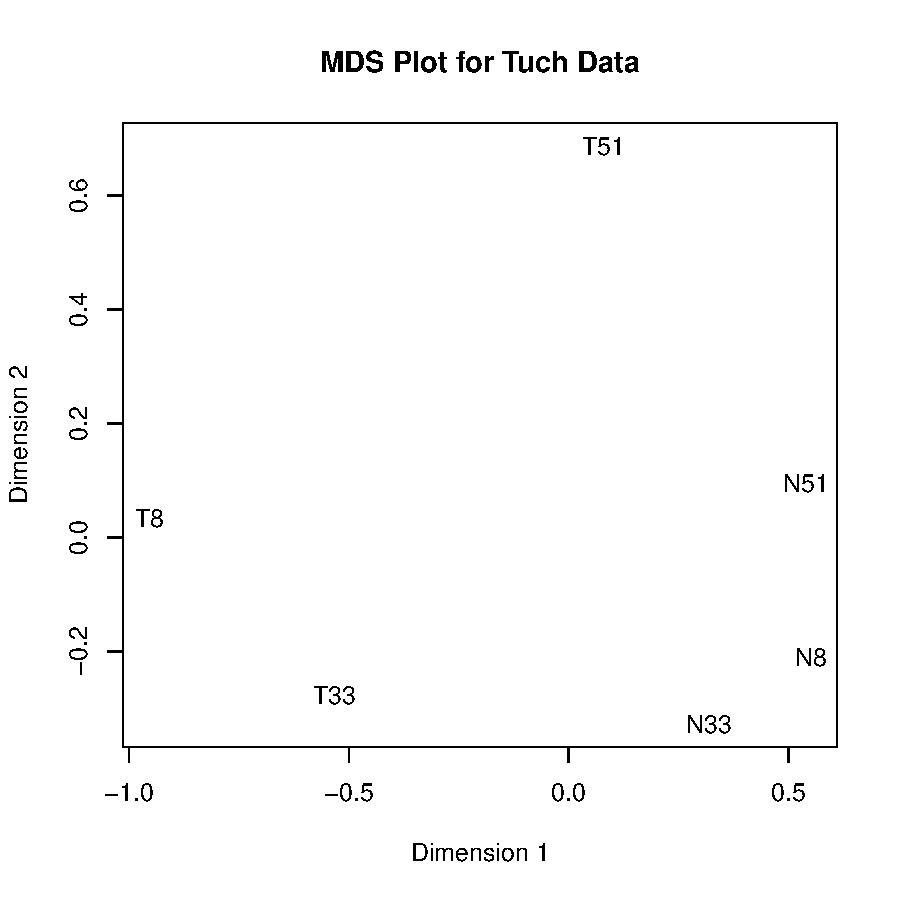
\includegraphics[height=0.45\textheight]{edgeR_case_study_Tuch_MDSplot}
\caption{Multidimensional scaling (MDS) plot for the Tuch data,
  showing the relations between the samples in two dimensions. From
  this plot, the samples T33 and T8 can be identified easily as outliers---there is a large distance between these two samples and the others.}
\label{fig:Tuch_MDS}
\end{center}
\end{figure}

\subsection{The design matrix}

Before we fit negative binomial GLMs, we need to define our design
matrix based on the experimental design. Here we want to test for
differential expressions between tumour and normal tissues within
patients, i.e.~adjusting for differences between patients. In
statistical terms, this is an additive linear model with patient as
the blocking factor. So the full design matrix can be created as
follows.

\begin{Schunk}
\begin{Sinput}
> patient <- factor(c(8, 8, 33, 33, 51, 51))
> design <- model.matrix(~patient + d.tuch$samples$group)
> rownames(design) <- rownames(d.tuch$samples)
> colnames(design)[4] <- "tumour"
> design
\end{Sinput}
\begin{Soutput}
    (Intercept) patient33 patient51 tumour
N8            1         0         0      0
T8            1         0         0      1
N33           1         1         0      0
T33           1         1         0      1
N51           1         0         1      0
T51           1         0         1      1
attr(,"assign")
[1] 0 1 1 2
attr(,"contrasts")
attr(,"contrasts")$patient
[1] "contr.treatment"

attr(,"contrasts")$`d.tuch$samples$group`
[1] "contr.treatment"
\end{Soutput}
\end{Schunk}

This is the design matrix under the alternative hypothesis (i.e.~the
difference between the normal tissue and the tumour tissue does
exist), and the design matrix under the null hypothesis is just the
above matrix without the last column.


\subsection{Analysis using Cox-Reid common dispersion}

\subsubsection{Estimating the Cox-Reid common dispersion}

The first major step in the analysis of DGE data using the NB model is
to estimate the dispersion parameter for each tag. Note that this is a
paired design experiment, so the dispersion has to be estimated in a
different way such that both the cell-type and the patient factors are
taken into account.

Like the qCML method (i.e.,the \code{estimateCommonDisp()} and the
\code{estimateTagwiseDisp()} function) we used in previous case
studies, the CR method also calculates both the common dispersion and
tagwise dispersions. The most straight-forward analysis for a paired
design experiment uses the CR common dispersion estimate as the
dispersion for all tags. For many applications this will be adequate
and it may not be necessary to estimate the CR tagwise dispersions,
i.e.~estimate the CR dispersion separately for each tag.

Estimating the CR common dispersion is done using the function
\code{estimateGLMCommonDisp()}. Once we have the design matrix, we
pass it to the \code{estimateGLMCommonDisp()} function, together
with the \code{DGEList} object `d.tuch'.
\begin{Schunk}
\begin{Sinput}
> d.tuch <- estimateGLMCommonDisp(d.tuch, design)
> names(d.tuch)
\end{Sinput}
\begin{Soutput}
[1] "samples"           "counts"            "genes"            
[4] "all.zeros"         "common.dispersion"
\end{Soutput}
\end{Schunk}

The output of \code{estimateCRDisp} is a \code{DGEList} object with
several new elements. The element \code{common.dispersion}, as the
name suggests, provides the estimate of the Cox-Reid common
dispersion, and \code{design} gives the design matrix as we defined at
the start.

Under the negative binomial model, the square root of the common
dispersion gives the coefficient of variation of biological
variation. Here the common dispersion is found to be
0.161, so the
coefficient of biological variation is around 0.401.

\begin{Schunk}
\begin{Sinput}
> d.tuch$common.dispersion
\end{Sinput}
\begin{Soutput}
[1] 0.160527
\end{Soutput}
\begin{Sinput}
> sqrt(d.tuch$common.dispersion)
\end{Sinput}
\begin{Soutput}
[1] 0.4006582
\end{Soutput}
\end{Schunk}

\subsubsection{Testing}
Once we have an estimate of the CR common dispersion, we can proceed
with testing procedures for determining differential expression. Since
this is a paired design experiment, we have to use the new testing
method, the GLM method, rather than the exact test (the one we
demonstrated in the previous case studies).

The GLM method fits a negative binomial generalized linear model for
each gene/tag with the unadjusted counts provided, a value for the
dispersion parameter and, optionally, offsets and weights for
different libraries or transcripts. This is done using the funtion
\code{glmFit()} and \code{glmLRT()}.

The function \code{glmFit()} calls the in-built function
\code{glm.fit()} to fit the NB GLM for each tag and produces an
object of class \code{DGEGLM}. Once we have a fit for a given design
matrix, \code{glmLRT()} can be run with a given coefficient or
contrast specified and evidence for differential expression can be
assessed using a likelihood ratio test. The \code{glmLRT} function
produces an object of class \code{DGELRT} with a table containing
the abundance of each tag (log-concentration, logConc), the log-fold
change of expression between conditions/contrasts being tested
(logFC), the likelihood ratio statistic (LR.statistic) and the p-value
from the LR test (p.value), for each tag in the dataset. Then tags can
be ranked in order of evidence for differential expression, based on
either the $p$-value or the log-fold change of expression computed for
each tag.

The results of the NB GLM likelihood ratio test can be accessed
conveniently using the \code{topTags} function applied to the object
produced by \code{glmLRT}. The user can specify the number,
\code{n}, of tags for which they would like to see the differential
expression information, ranked by $p$-value (default) or fold
change. As the same test is conducted for many thousands of tags,
adjusting the $p$-values for multiple testing is recommended. The
desired adjustment method can be supplied by the user, with the
default method being Benjamini and Hochberg's approach for controlling
the false discovery rate (FDR)~\citep{Benjamini95}. The table below
shows the top $10$ DE genes ranked by $p$-value.

\begin{Schunk}
\begin{Sinput}
> glmfit.tuch <- glmFit(d.tuch, design, dispersion = d.tuch$common.dispersion)
> lrt.tuch <- glmLRT(d.tuch, glmfit.tuch, coef = 4)
> options(digits = 4)
> topTags(lrt.tuch)
\end{Sinput}
\begin{Soutput}
Coefficient:  tumour 
                 genes logConc  logFC     LR   P.Value       FDR
NM_182502    TMPRSS11B  -8.506 -7.322 121.55 2.892e-28 3.026e-24
NM_016190         CRNN  -6.987 -7.256 107.46 3.538e-25 1.851e-21
NM_002371          MAL  -8.952 -6.810 106.38 6.089e-25 2.124e-21
NM_002465       MYBPC1  -8.157 -7.019  99.75 1.727e-23 4.518e-20
NM_014440        IL1F6 -10.060 -6.148  96.06 1.114e-22 2.332e-19
NM_002272         KRT4  -5.621 -7.133  92.79 5.800e-22 9.311e-19
NM_001010909     MUC21  -8.797 -6.724  92.65 6.229e-22 9.311e-19
NM_001100        ACTA1  -8.390 -6.281  92.08 8.329e-22 1.089e-18
NM_003280        TNNC1  -9.188 -6.958  91.38 1.186e-21 1.379e-18
NM_006063      KBTBD10  -8.232 -6.215  89.07 3.813e-21 3.990e-18
\end{Soutput}
\end{Schunk}

The output shows that the \edgeR~package identifies a good deal of
differential expression between the normal tissue group and the tumour
tissue group. The top DE tags are given very small $p$-values, even
after adjusting for multiple testing. Furthermore, all of the top tags
have a large fold change, indicating that these tags are more likely
to be biologically meaningful.

The table below shows the raw counts for the tags that \edgeR~has
identified as the most differentially expressed. For these tags there
seems to be very large differences between the groups, suggesting that
the DE tags identified are truly differentially expressed, and not
false positives.

\begin{Schunk}
\begin{Sinput}
> top <- rownames(topTags(lrt.tuch)$table)
> d.tuch$counts[top, order(d.tuch$samples$group)]
\end{Sinput}
\begin{Soutput}
                N8   N33   N51  T8   T33  T51
NM_182502     2592  7805  3372   3   321    9
NM_016190    24146 22026 12480  49  2353   26
NM_002371     2697  3941  1750   3   265    8
NM_002465     4809  4146 15623  10    14 1311
NM_014440      367  1824   802  10    45    1
NM_002272    76461 99082 47411 353 20651   31
NM_001010909  4160  3425  1720   7   516    5
NM_001100     3334  3198 13643   8    32 1063
NM_003280     1684  1787  4894   0     7  559
NM_006063     4325  3115 16007  24    17 1461
\end{Soutput}
\end{Schunk}

Note that the 2nd tag ('CKM') and the 7th tag ('MYBPC1') have much
larger counts in patient 55 than in the other two patients, which
shows that the effect from the patients does exist and the GLM method
can pick that up.

If we order the genes by fold change instead of $p$-value, as in the
table below, we see that the tags with the largest fold changes have
very small concentrations. This ranking is dominated by genes that
have zero counts in one group and is less informative than ranking by
$p$-value.

\begin{Schunk}
\begin{Sinput}
> topTags(lrt.tuch, sort.by = "logFC")
\end{Sinput}
\begin{Soutput}
Coefficient:  tumour 
                 genes logConc  logFC     LR   P.Value       FDR
NM_001100112      MYH2  -8.126 -7.347  86.96 1.107e-20 1.053e-17
NM_182502    TMPRSS11B  -8.506 -7.322 121.55 2.892e-28 3.026e-24
NM_016190         CRNN  -6.987 -7.256 107.46 3.538e-25 1.851e-21
NM_002272         KRT4  -5.621 -7.133  92.79 5.800e-22 9.311e-19
NM_002465       MYBPC1  -8.157 -7.019  99.75 1.727e-23 4.518e-20
NM_003280        TNNC1  -9.188 -6.958  91.38 1.186e-21 1.379e-18
NM_152381        XIRP2  -7.427 -6.927  75.86 3.049e-18 9.969e-16
NM_002371          MAL  -8.952 -6.810 106.38 6.089e-25 2.124e-21
NM_001010909     MUC21  -8.797 -6.724  92.65 6.229e-22 9.311e-19
NM_198060         NRAP  -8.451 -6.441  82.70 9.543e-20 5.548e-17
\end{Soutput}
\begin{Sinput}
> top <- rownames(topTags(lrt.tuch, sort.by = "logFC")$table)
> d.tuch$counts[top, order(d.tuch$samples$group)]
\end{Sinput}
\begin{Soutput}
                N8   N33   N51  T8   T33  T51
NM_001100112  4389  7944  9262   7    16 1818
NM_182502     2592  7805  3372   3   321    9
NM_016190    24146 22026 12480  49  2353   26
NM_002272    76461 99082 47411 353 20651   31
NM_002465     4809  4146 15623  10    14 1311
NM_003280     1684  1787  4894   0     7  559
NM_152381     9915 10396 23309  15    48 7181
NM_002371     2697  3941  1750   3   265    8
NM_001010909  4160  3425  1720   7   516    5
NM_198060     3741  1990 12531   4    17 1829
\end{Soutput}
\end{Schunk}


We see in the output below that over $1200$ tags are significantly
differentially expressed according to \edgeR~when using the CR common
dispersion estimate and GLM likelihood ratio test. Of those tags,
$297$ are up-regulated in the tumour tissues compared with the normal
tissues and $975$ are down-regulated in the tumour tissues compared
with normal tissues.

\begin{Schunk}
\begin{Sinput}
> summary(decideTestsDGE(lrt.tuch))
\end{Sinput}
\begin{Soutput}
   [,1]
-1  975
0  9192
1   297
\end{Soutput}
\end{Schunk}


\subsection{Cox-Reid dispersions with mean-dependent trend}
\label{sec:cox-reid-dispersions}

It has been noted that the dispersion parameter in RNA-seq data can
depend on the expression level of the gene \citep{Anders:2010p792}. The
function \code{estimateGLMTrendedDisp} in \edgeR~estimates
dispersion values that depend on the overall expression level of the
genes. Typically, lowly expressed genes have a higher value for the
dispersion parameter than more highly expressed genes. There are a
number of possible options for the type of trend that is to be fit for
the dispersion parameters. These options are detailed in the help file
for \code{estimateGLMTrendedDisp}.

\begin{Schunk}
\begin{Sinput}
> d.tuch <- estimateGLMTrendedDisp(d.tuch, design)
> summary(d.tuch$trended.dispersion)
\end{Sinput}
\begin{Soutput}
   Min. 1st Qu.  Median    Mean 3rd Qu.    Max. 
  0.124   0.129   0.150   0.162   0.172   0.558 
\end{Soutput}
\end{Schunk}

An analysis could be carried out just as for the common dispersion
above, but is not shown here.


\subsection{Analysis using Cox-Reid tagwise dispersion}


\subsubsection{Estimating the Cox-Reid tagwise dispersion}

An extension to simply using the CR common dispersion for each tag is
to estimate the CR dispersion separately for each tag, while
`squeezing' these estimates towards the CR common dispersion estimate
in order to improve inference by sharing information between
tags. This type of analysis can also be carried out in few steps using
the \edgeR~package.

As noted earlier, the dispersion parameter is the overdispersion
relative to the Poisson, and represents the biological, or
sample-to-sample variability. The methods we have developed moderate
the dispersion estimates towards a common dispersion, much like how
the \limma~package moderates the variances in the analysis of
microarray data.

The amount of moderation done is determined by the value of a weight
parameter \code{prior.n}. The value for \code{prior.n} corresponds to
the number of individual tags equivalent to the weight given to the
common likelihood. Thus, the higher \code{prior.n}, the more strongly
the individual dispersion estimates are moderated, or `squeezed',
towards the common value. To run the moderated analysis, we need to
determine how much moderation is necessary. How best to do this is
still an open research question, but we currently recommend selecting
a value for the weight parameter \code{prior.n} \emph{a priori} and
have found that very good results can be obtained this way.

In an experiment such as that we consider here, in which we have just
six samples, with two groups (group factor) and three patients
(blocking factor), and thus two degrees of freedom for estimating the
dispersion parameter. Standard tagwise dispersion estimates are likely
to be unreliable, so we want to give a reasonable weight to the common
likelihood. We need to choose a value for \code{prior.n} such that
individual tagwise dispersion estimates are `squeezed' quite strongly
towards the common dispersion. Here, we choose a moderate amount of
smoothing---we let \code{prior.n} be $8$. This means that the common
likelihood receives the weight of $8$ individual tags, so there will
be a reasonable degree of `squeezing', but there is still ample scope
to estimate an individual dispersion for each tag.

The function \code{estimateGLMTagwiseDisp} adds the CR tagwise
dispersion estimates to the DGEList object provided as an argument.

\begin{Schunk}
\begin{Sinput}
> d.tuch <- estimateGLMTagwiseDisp(d.tuch, design, prior.n = 8)
> names(d.tuch)
\end{Sinput}
\begin{Soutput}
 [1] "samples"            "counts"             "genes"             
 [4] "all.zeros"          "common.dispersion"  "trended.dispersion"
 [7] "abundance"          "bin.dispersion"     "bin.abundance"     
[10] "tagwise.dispersion"
\end{Soutput}
\begin{Sinput}
> head(d.tuch$tagwise.dispersion)
\end{Sinput}
\begin{Soutput}
NM_000014 NM_144670 NM_017436 NM_015665 NM_023928 NM_024666 
   0.1933    0.2415    0.2051    0.1528    0.1157    0.1246 
\end{Soutput}
\end{Schunk}

It is interesting to consider the distribution of the CR tagwise
dispersion estimates. As we can see from the output below, the CR
tagwise dispersion estimates range from a minimum of $0.11$ to a
maximum of $0.69$. The range of dispersions is therefore large, but
the tags in the middle two quartiles of the CR tagwise dispersion
estimates have dispersion estimates close to the CR common dispersion
estimate.

\begin{Schunk}
\begin{Sinput}
> summary(d.tuch$tagwise.dispersion)
\end{Sinput}
\begin{Soutput}
   Min. 1st Qu.  Median    Mean 3rd Qu.    Max. 
  0.110   0.125   0.148   0.161   0.172   0.686 
\end{Soutput}
\end{Schunk}

\subsubsection{Testing}
The testing procedures when using CR tagwise dispersion estimates are
carried out exactly as for the CR common dispersion, as described
above. Here we carry out the testing using the CR tagwise dispersion
estimates calculated using a \code{prior.n} value of eight. The GLM fit
and the likelihood ratio test are done using the same functions as
before (i.e.~\code{glmFit()} and \code{glmLRT()}), the only
difference is that we use CR tagwise dispersions as the dispersion in
the \code{glmFit()} function.

\begin{Schunk}
\begin{Sinput}
> glmfit.tuch.tgw <- glmFit(d.tuch, design, dispersion = d.tuch$tagwise.dispersion)
> lrt.tuch.tgw <- glmLRT(d.tuch, glmfit.tuch.tgw)
\end{Sinput}
\end{Schunk}

The output below shows that when using CR tagwise dispersions, the
\edgeR~package still identifies a lot of differential expression
between the normal tissue group and the tumour tissue group. This
arises because the moderated tagwise dispersions can be much smaller
than the common dispersion, and tags with smaller dispersions will
have smaller $p$-values than the same tags with $p$-values computed
using a common dispersion. As with the analysis using the common
dispersion, all of the top tags have a large fold change, indicating
that these changes in expression are likely to be biologically
meaningful. We note that the ranking is different, however, and not
all of the top ten tags according to using the common dispersion are
found to be among the top ten tags using tagwise dispersions.

\begin{Schunk}
\begin{Sinput}
> options(digits = 4)
> topTags(lrt.tuch.tgw)
\end{Sinput}
\begin{Soutput}
Coefficient:  tumour 
                 genes logConc  logFC     LR   P.Value       FDR
NM_014440        IL1F6 -10.060 -6.142 100.20 1.374e-23 1.438e-19
NM_001039585     PTGFR -10.519 -5.193  95.02 1.883e-22 9.854e-19
NM_005609         PYGM  -9.653 -5.476  89.85 2.567e-21 8.955e-18
NM_182502    TMPRSS11B  -8.506 -7.412  87.33 9.182e-21 2.402e-17
NM_004533       MYBPC2  -9.299 -5.458  82.56 1.027e-19 2.150e-16
NM_004320       ATP2A1  -9.669 -4.622  78.52 7.920e-19 1.381e-15
NM_002371          MAL  -8.952 -6.902  76.58 2.117e-18 2.961e-15
NM_057088         KRT3  -9.301 -5.838  76.45 2.264e-18 2.961e-15
NM_001111283      IGF1  -9.841 -3.992  75.10 4.464e-18 5.191e-15
NM_001976         ENO3  -9.423 -5.179  73.12 1.218e-17 1.275e-14
\end{Soutput}
\end{Schunk}

The table below shows the raw counts for the tags that \edgeR~has
identified as the most differentially expressed using CR tagwise
dispersions. For these tags there seems to be very large differences
between the groups, suggesting that the DE tags identified are truly
differentially expressed, and not false positives.

\begin{Schunk}
\begin{Sinput}
> top.tgw <- rownames(topTags(lrt.tuch.tgw)$table)
> d.tuch$counts[top.tgw, order(d.tuch$samples$group)]
\end{Sinput}
\begin{Soutput}
               N8  N33  N51 T8 T33 T51
NM_014440     367 1824  802 10  45   1
NM_001039585  455  287 1736  7  12  46
NM_005609    1399 1267 2171 22  16 103
NM_182502    2592 7805 3372  3 321   9
NM_004533     966  486 8045 11   6 457
NM_004320     988 1558 2285 25  52 161
NM_002371    2697 3941 1750  3 265   8
NM_057088    1069 3774  885  7 358   5
NM_001111283  460  343 4703 25  26 257
NM_001976    1092 1292 4841  4  74 223
\end{Soutput}
\end{Schunk}

We see in the output below that $1272$ tags are significantly
differentially expressed according to \edgeR~when using the CR tagwise
dispersion estimate and GLM likelihood ratio test. It is slightly less
the total number of DE tags under the CR common dispersion method. Of
those $1272$ tags, $313$ are up-regulated in the tumour tissues
compared with the normal tissues and $959$ are down-regulated in the
tumour tissues compared with normal tissues.

\begin{Schunk}
\begin{Sinput}
> summary(decideTestsDGE(lrt.tuch.tgw))
\end{Sinput}
\begin{Soutput}
   [,1]
-1  959
0  9192
1   313
\end{Soutput}
\end{Schunk}


\subsection{Setup}
This analysis of \citet{Tuch:2010p457}'s RNA-seq data was conducted on:
\begin{Schunk}
\begin{Sinput}
> sessionInfo()
\end{Sinput}
\begin{Soutput}
R version 2.13.0 beta (2011-03-30 r55205)
Platform: i386-apple-darwin9.8.0/i386 (32-bit)

locale:
[1] C/UTF-8/C/C/C/C

attached base packages:
[1] splines   stats     graphics  grDevices utils     datasets  methods  
[8] base     

other attached packages:
[1] org.Hs.eg.db_2.5.0    RSQLite_0.9-4         DBI_0.2-5            
[4] AnnotationDbi_1.13.18 Biobase_2.11.10       limma_3.7.26         
[7] edgeR_2.1.17         

loaded via a namespace (and not attached):
[1] tools_2.13.0
\end{Soutput}
\end{Schunk}


